

%%%
%%%  FIGURE 
%%%
\begin{figure}[h]
%\vspace{-1.cm}
%\vbox{

%\begin{center}
%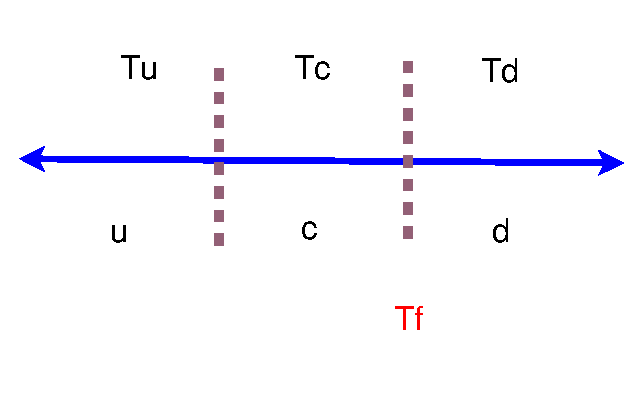
\includegraphics[width=0.6\textwidth]{1D_Sketch_b.eps}
%\vspace{-1.cm}
%\end{center}
%\hbox{\hspace{6.5cm}(a)}
%\vspace{.1cm}
%
%\begin{center}
%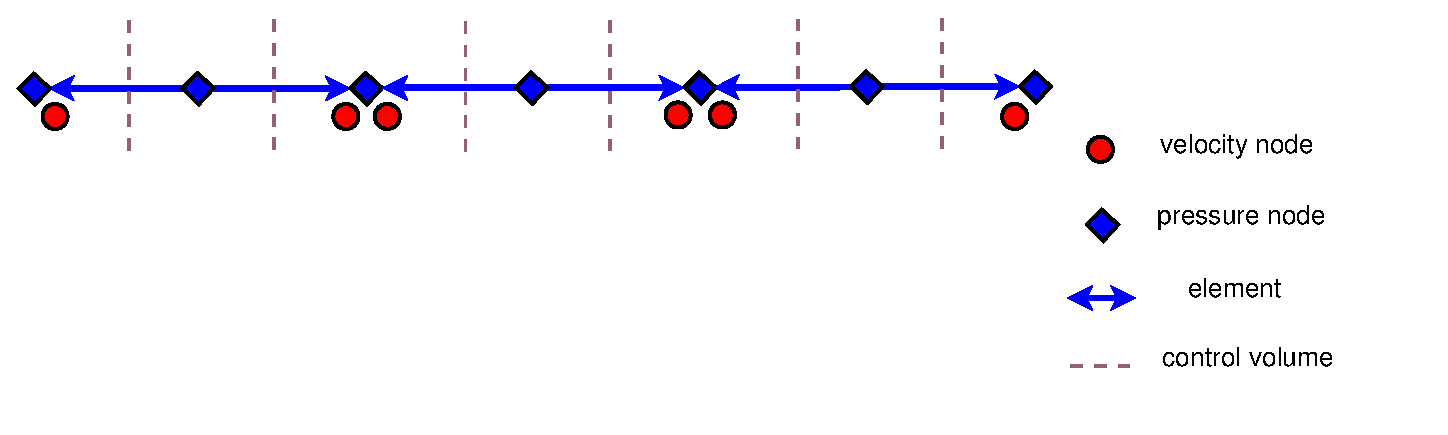
\includegraphics[width=1.\textwidth]{1D_Sketch.eps}
%\vspace{-1.cm}
%\end{center}
%\hbox{\hspace{6.5cm}(b)}
%\vspace{-.1cm}



\vbox{
\hbox{ \hspace{4.cm}
\includegraphics[width=.55\textwidth]{diagrams/p0dgp1-cont-sat} \hspace{0.cm} (a)}
\vspace{-0.2cm}
\hbox{ \hspace{4.cm}
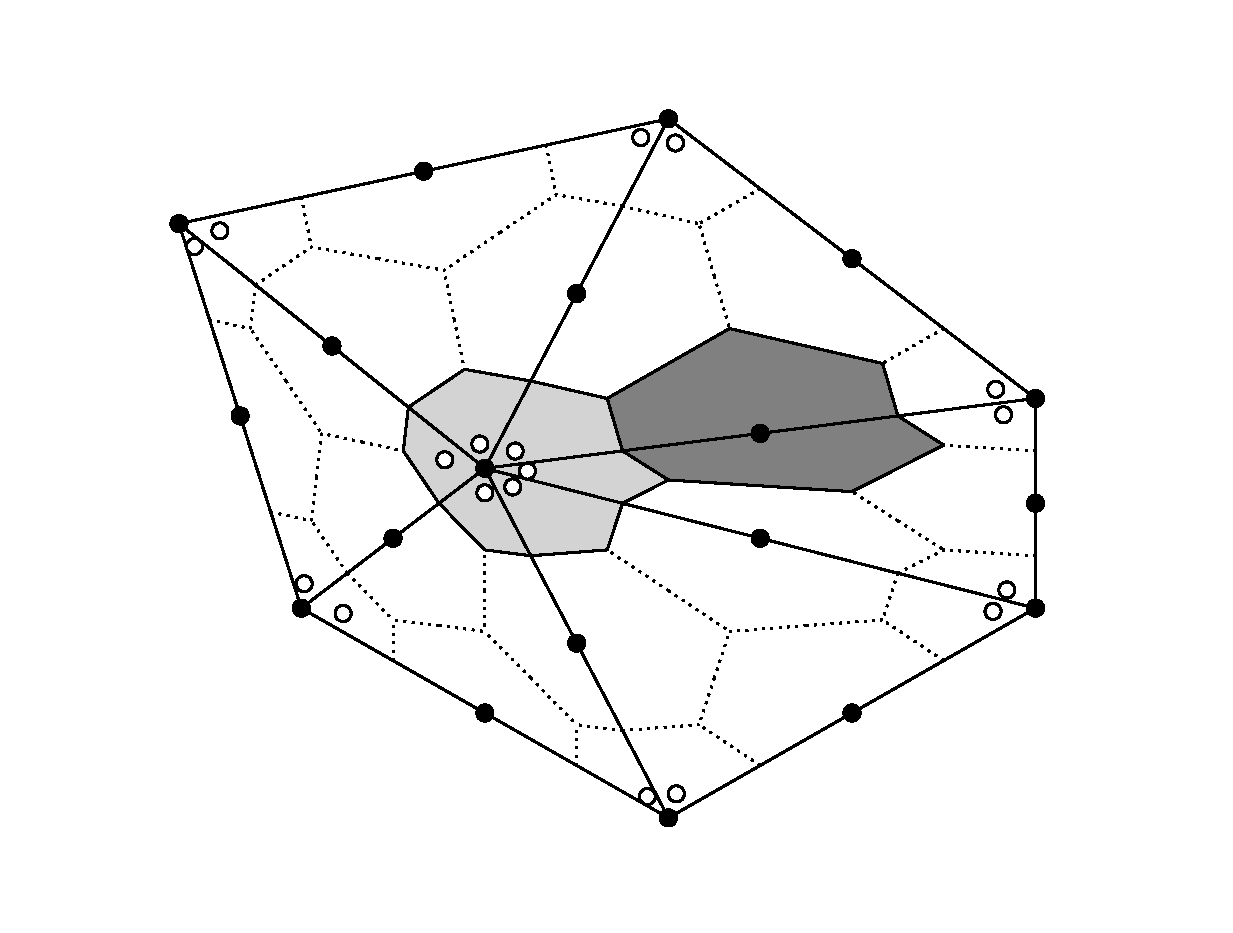
\includegraphics[width=.55\textwidth]{diagrams/p1dgp2-cont-sat} \hspace{0.cm} (b)}
\vspace{-0.2cm}
\hbox{ \hspace{4.cm}
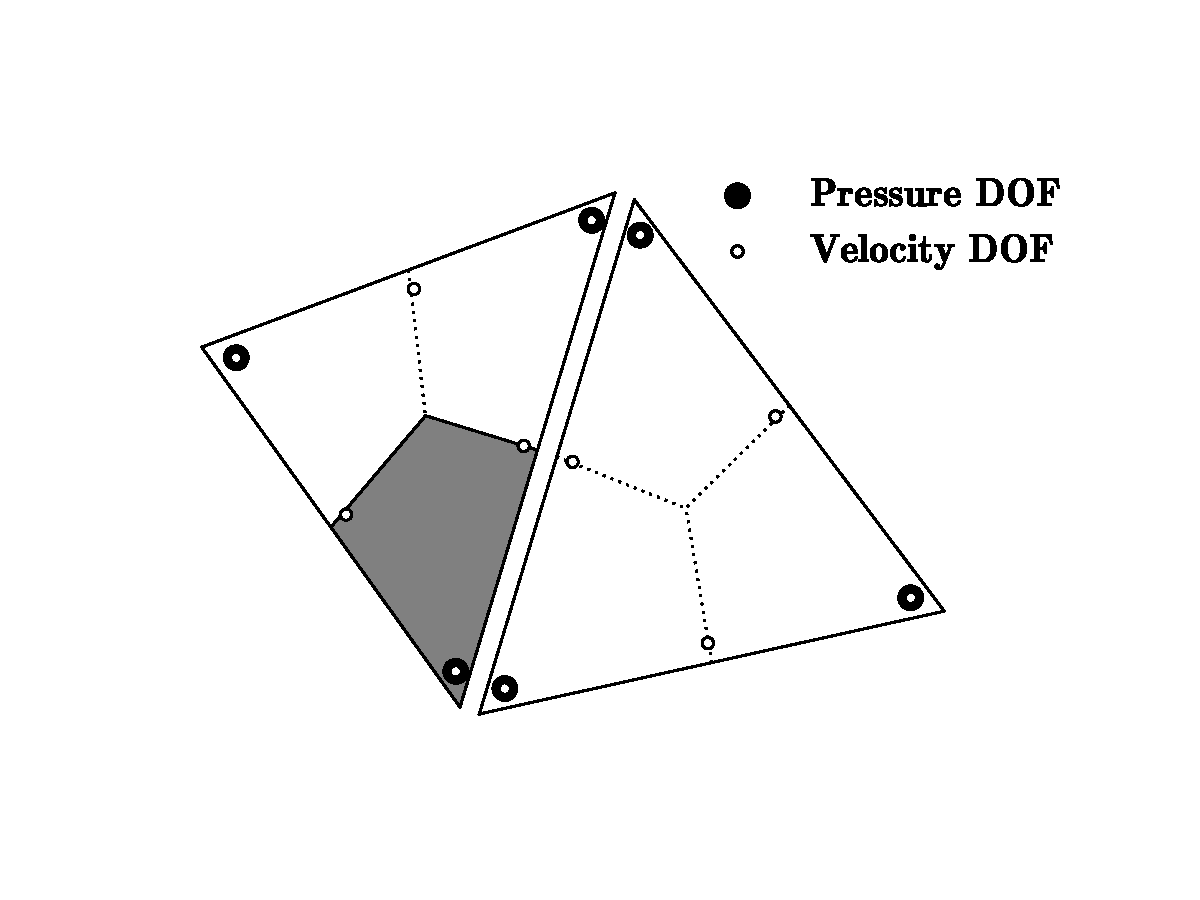
\includegraphics[width=.55\textwidth]{diagrams/p2dgp1-dg-sat} \hspace{0.cm} (c)}
\vspace{-0.2cm}

%\vspace{.1cm}
}

  \caption{2D representation of the element pairs (a) P0DGP1, (b) P1DGP2  and (c) P2DGP1DG. Shaded areas denote a control volumes (in which saturation is stored), black points represent the pressure nodes and the white points the velocity.}
  \label{fem_cv_represent_a}
\end{figure}


%%%
%%% Overlapping Figure 1
%%%

\begin{figure}[htp]
\begin{center}
\hbox{\hspace{-2.cm}
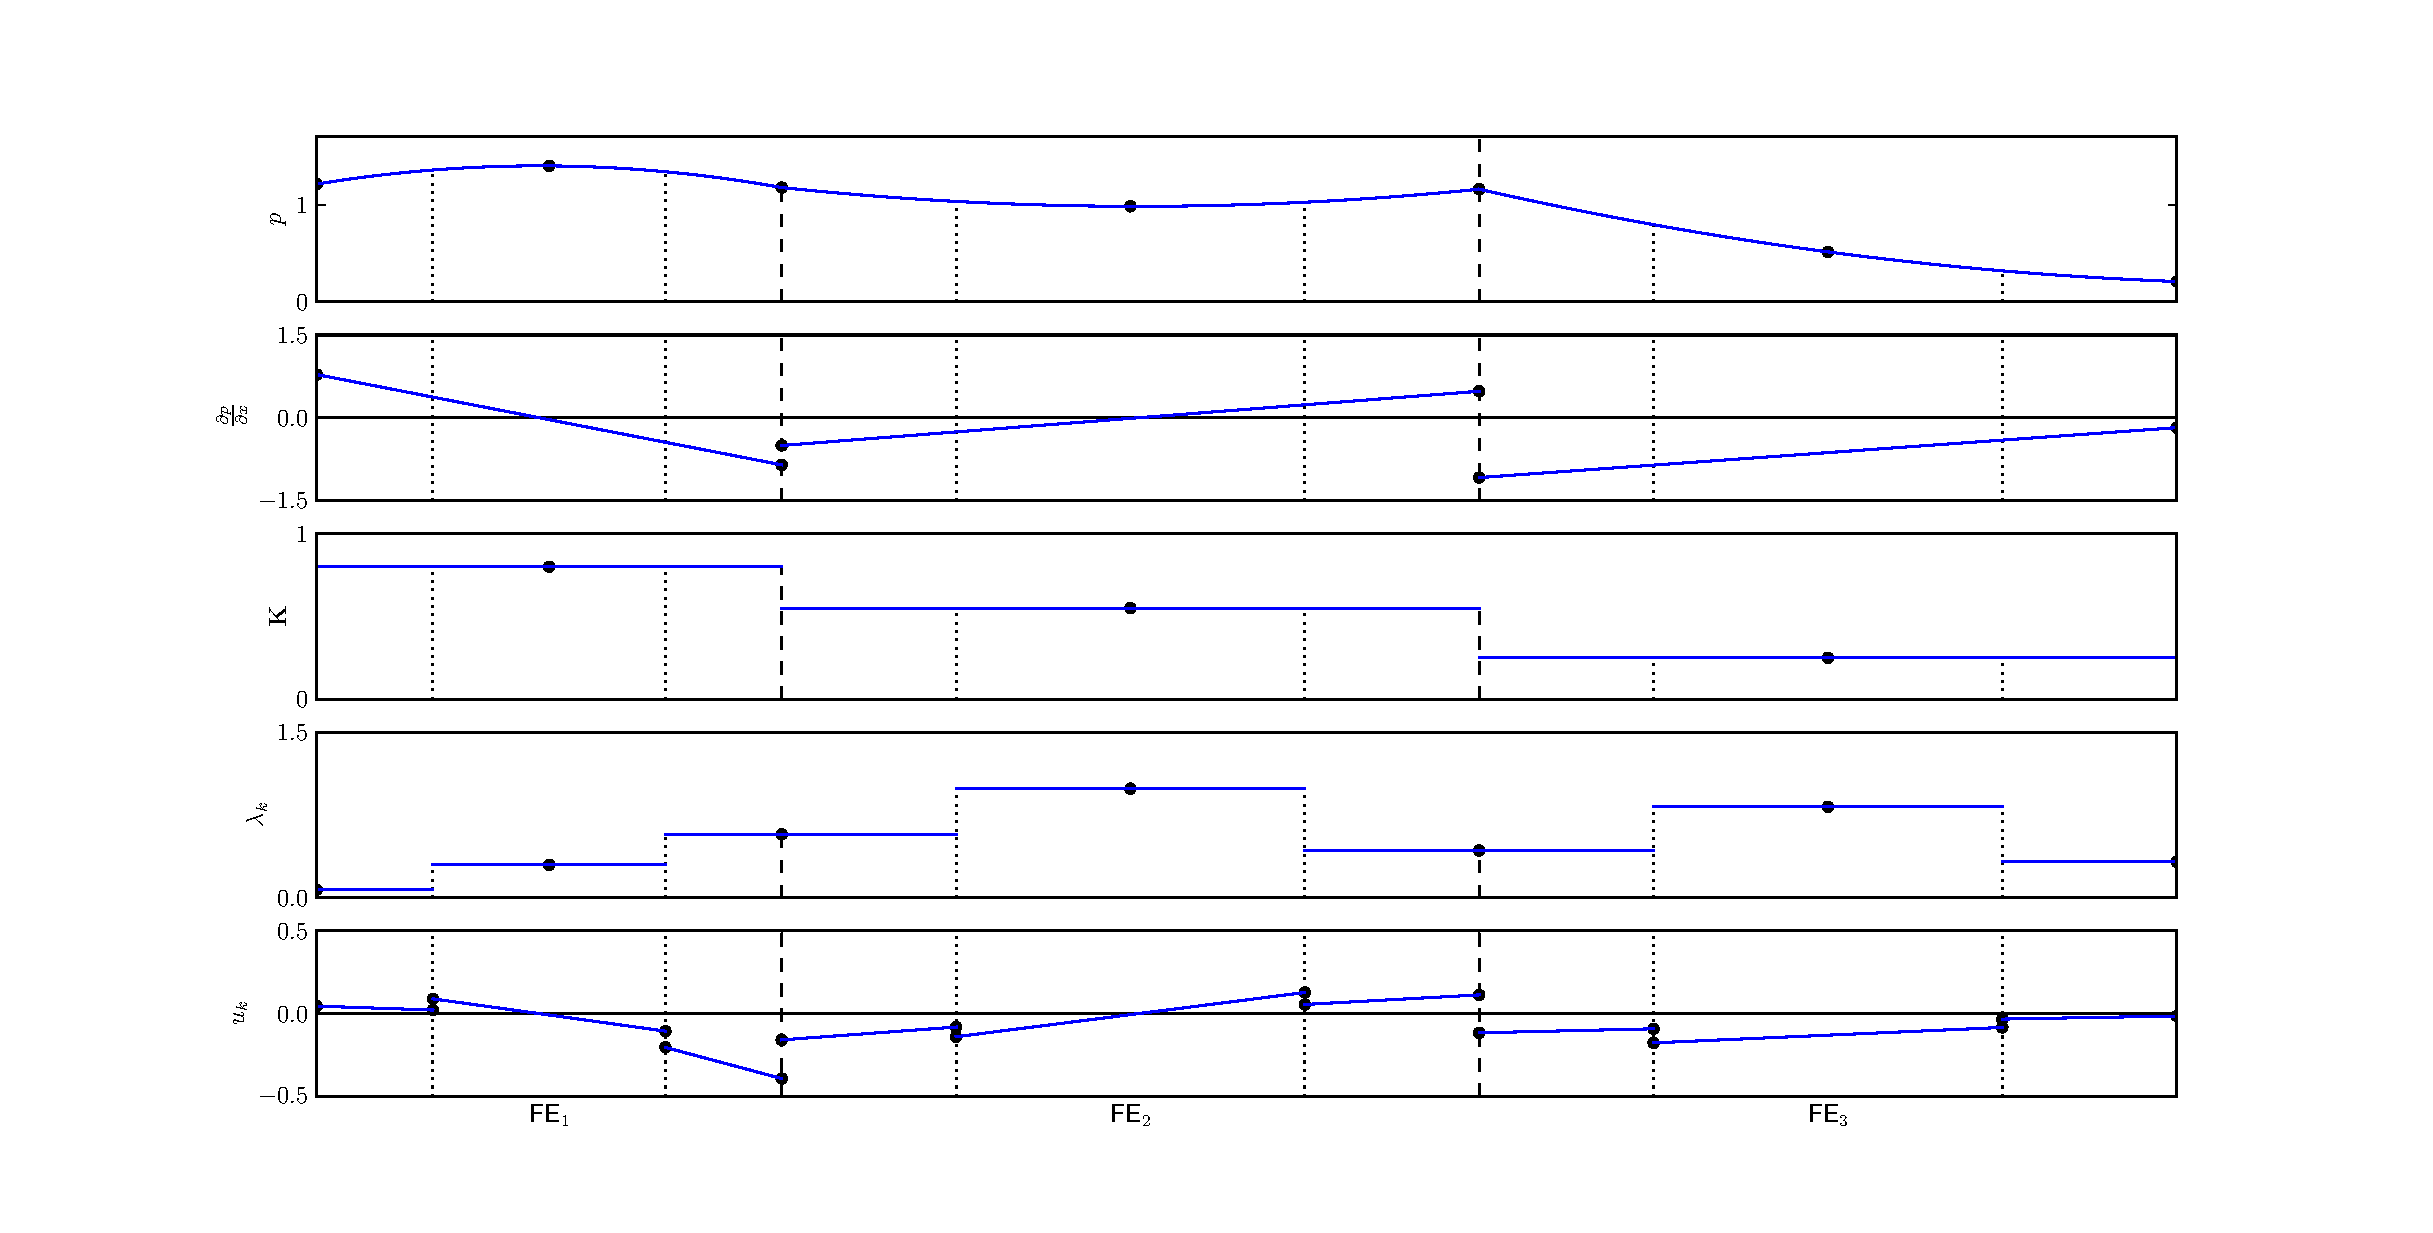
\includegraphics[width=1.3\textwidth,height=1.3\textwidth]{diagrams/overlapping_cartoon}}
\vspace{-1.4cm}
\caption{Diagram showing the exact representation of Darcy's law in 1D. From top to bottom, the plots show i) a P2 continuous pressure field, $p$, across three elements, ii) the P1DG gradient of that  pressure field, iii) a P0DG absolute permeability field, ${\bf K}$, iv) a CV mobility field, $\lambda_{k}=\frac{\mathcal{K}_{rk}\left(S_{k}\right)}{\mu_{k}}$, and finally v) the resultant CV0DG velocity field arising from Darcy's law. Here dashed lines denote the boundaries of the P2 finite element mesh, dotted lines denote boundaries between the control volumes dual to the P2 mesh and solid dots indicate the natural locations of degrees of freedom in a non-overlapping formulation. }
\label{fig:darcys_law}
\end{center}
\end{figure}

%%%
%%% Overapping Figure 2
%%%

\begin{figure}[htp]
\begin{center}
\hbox{\hspace{-2.5cm}
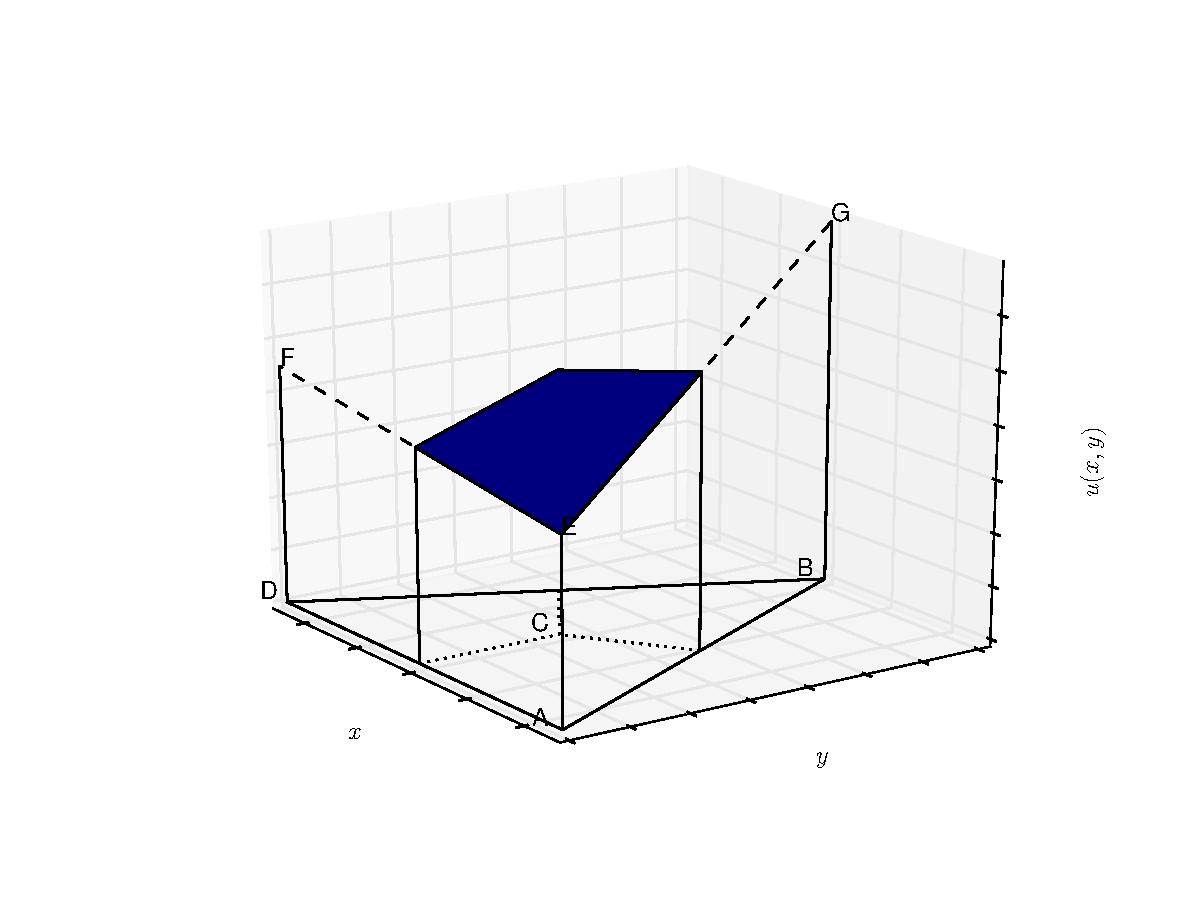
\includegraphics[width=1.2\textwidth]{diagrams/overlapping}}
\caption{An isometric schematic of the 2D overlapping velocity
  elements. In this example we show a triangular element, ABD in the
  $x$-$y$ plane. We also indicate the contol volume boundaries lying
  within this element. Under the overlapping methodology presented
  here, each facet formed from the union of control volume and element
  possesses its own polynomial representation for velocity, indicated
  by height in the isometric projection. By extrapolating this
  representation across the rest of this element, we negate the need
  to implement a special data structure to store or evaluate this
  field, instead leveraging the standard finite element basis for ABD,
  and storing the FEM nodal values E, F, G. }
\label{fig:overlapping2d}
\end{center}
\end{figure}


%%%
%%%  FIGURE 
%%%
%\begin{figure}[H]
%\vbox{
%\begin{center}
%\includegraphics[width=10.0cm,height=7.5cm]{FEM_elem2}
%\end{center}
%\vspace{-3.cm}}
%\caption{Positioning of variables in and on the boundary of CV {\it i}.}
%\label{fem_cv_represent_c}
%\end{figure}



%%%
%%%  FIGURE 
%%%
\begin{figure}[h]
 
  \begin{center}
\vbox{\hbox{\hspace{1cm}
    \includegraphics[width=0.8\textwidth]{compar-dg.eps}}
   \hbox{ \hspace{1cm} \includegraphics[width=0.8\textwidth]{compar-dg-bdt.eps}}}
    \caption{Advection problem test-cases: control volume solution (5
      finite elements with constant width of 0.2 are used) with
      Courant number of 0.005 (top) and 0.5 (bottom).  The solution
      has been advected a distance of 0.2 with 200 (top) and 2
      (bottom) time steps. The 50 elements solution is shown to give
      an indication of the accuracy of the solutions and has a Courant
      number (based on the element width) of 0.005.\label{compar-dg}}
  \end{center}
\end{figure}

%%%
%%%  FIGURE 
%%%
\begin{figure}[h]
\begin{center}
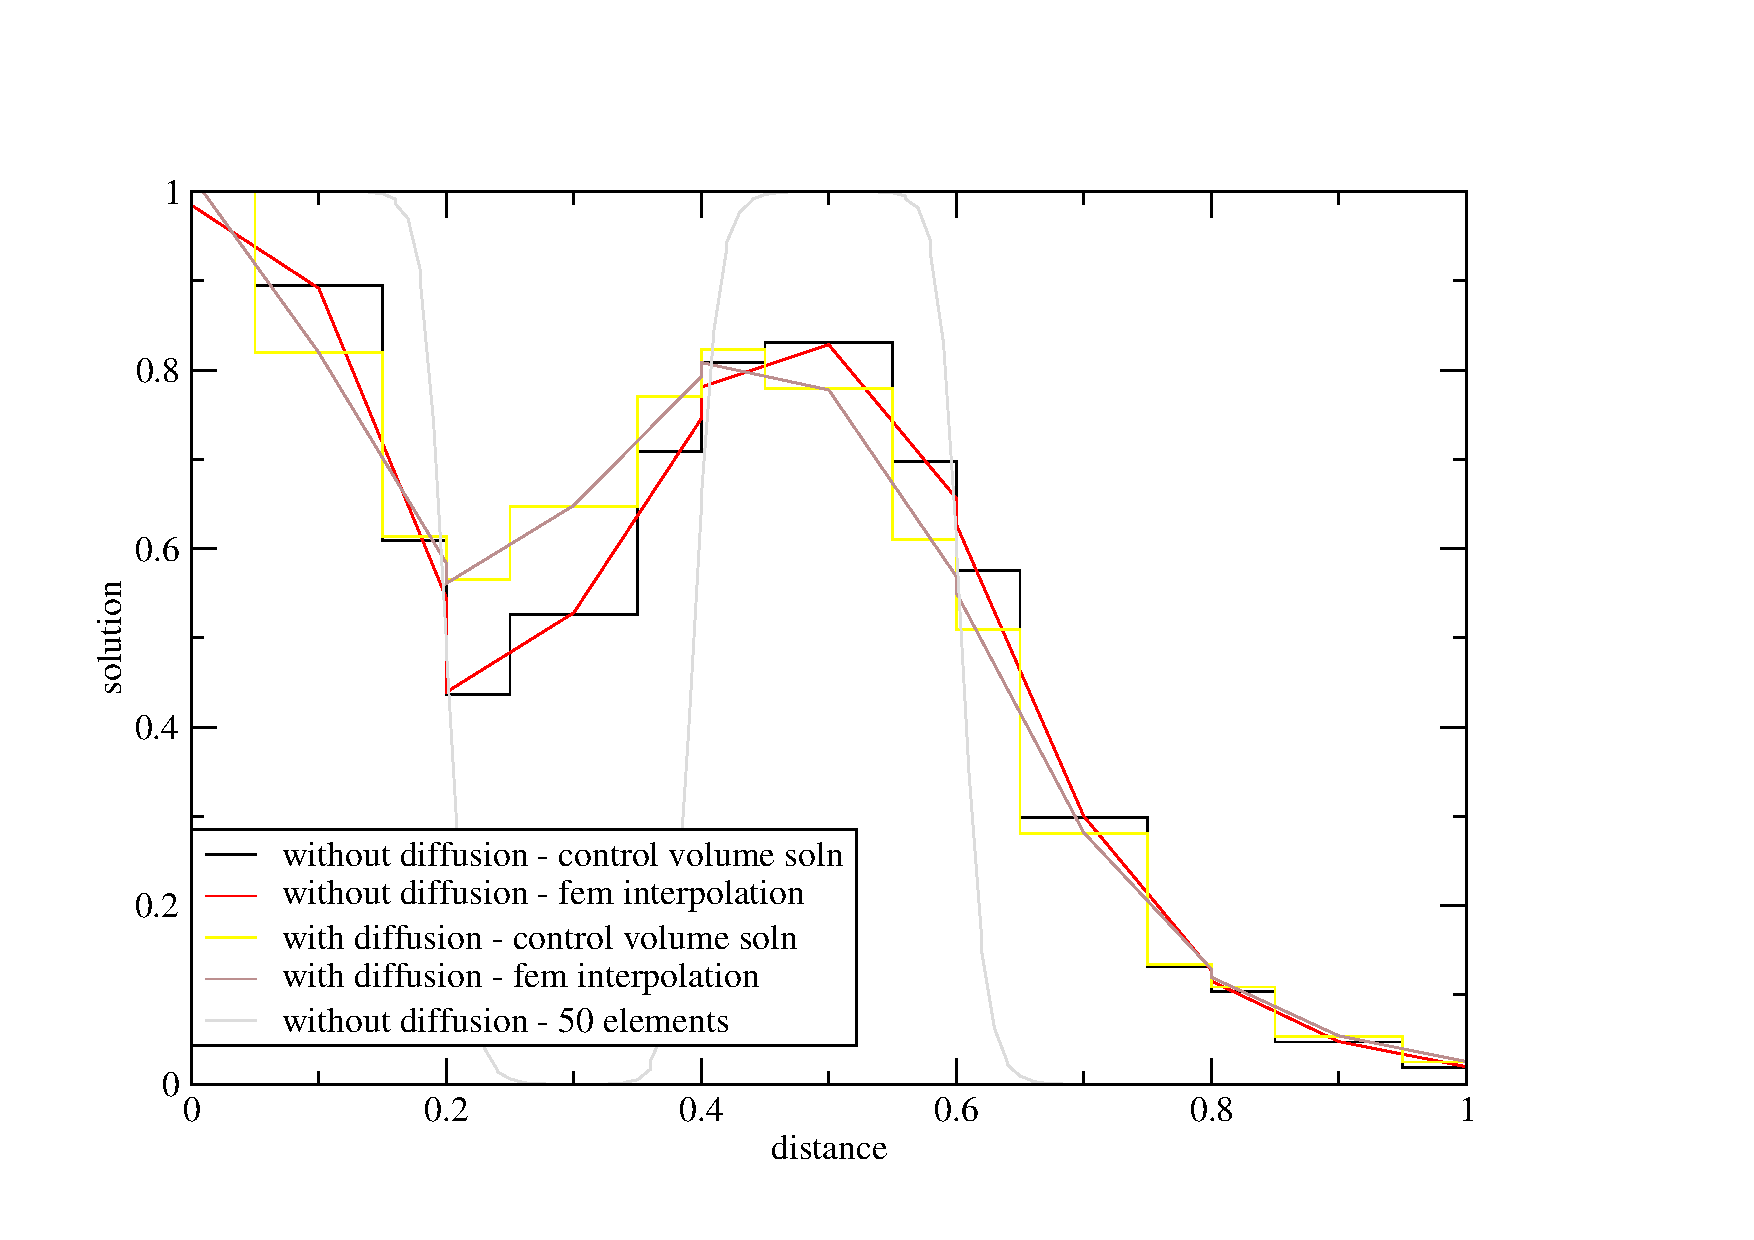
\includegraphics[width=1.2\textwidth]{compar-dg-bdt-diff}
\end{center}
\caption{Advection problem test-cases: discontinuous (between
  elements) control volume formulation within 5 finite elements (width
  of 0.2). Courant number is of 0.5 (or 2 if based on the minimum
  width of a control volume). The solution has been advected a
  distance of 0.2 with 2 time steps. The 50 element solution is for
  pure advection and is shown to give an indication of the accuracy of
  the solutions and has a Courant number (based on the element width)
  of 0.005.\label{compar-dg-bdt-diff}}
\end{figure}


%%%
%%%  FIGURE 
%%%
\begin{figure}[h]
\vbox{\hbox{\hspace{-1.3cm}
\includegraphics[width=17.5cm,height=12.5cm]{theta-bdt}}
\vspace{0.cm}}
\caption{Advection problem test-cases: value of $\theta$-time stepping
  parameter on the faces of the control volumes at the end of the
  simulation -- 5 FE are used and the Courant number (based on the
  element width of 0.2) is 0.5 (or 2 if based on the minimum width of
  a control volume). The solution has been advected a distance of 0.2
  length units with 2 time steps.}
\label{theta-bdt}
\end{figure}


%%%
%%%  FIGURE 
%%%
\begin{figure}[h]
\vbox{\vspace{-2cm}
\hbox{\hspace{-.5cm}
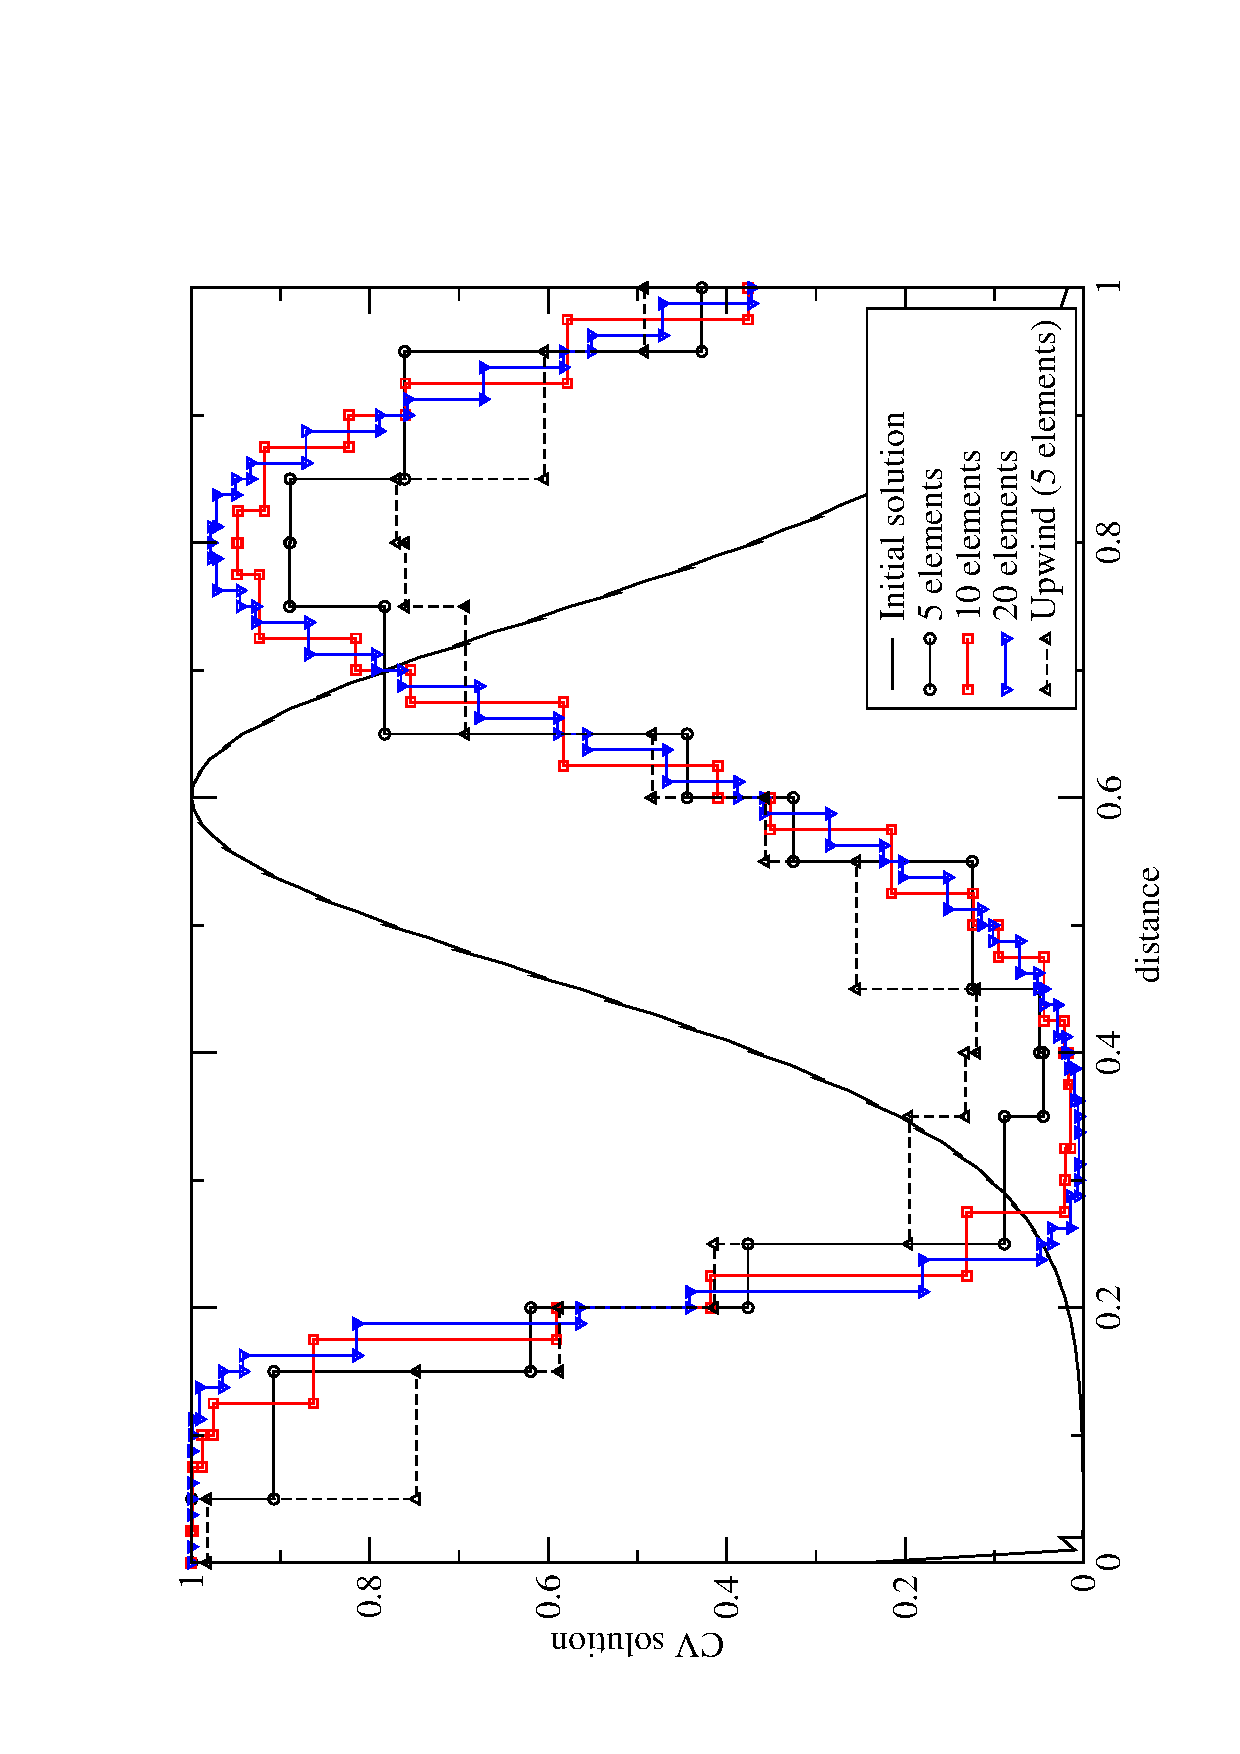
\includegraphics[width=14.0cm,height=10.cm]{converg-cv}}
\vspace{-.5cm}
\hbox{\hspace{-.5cm}
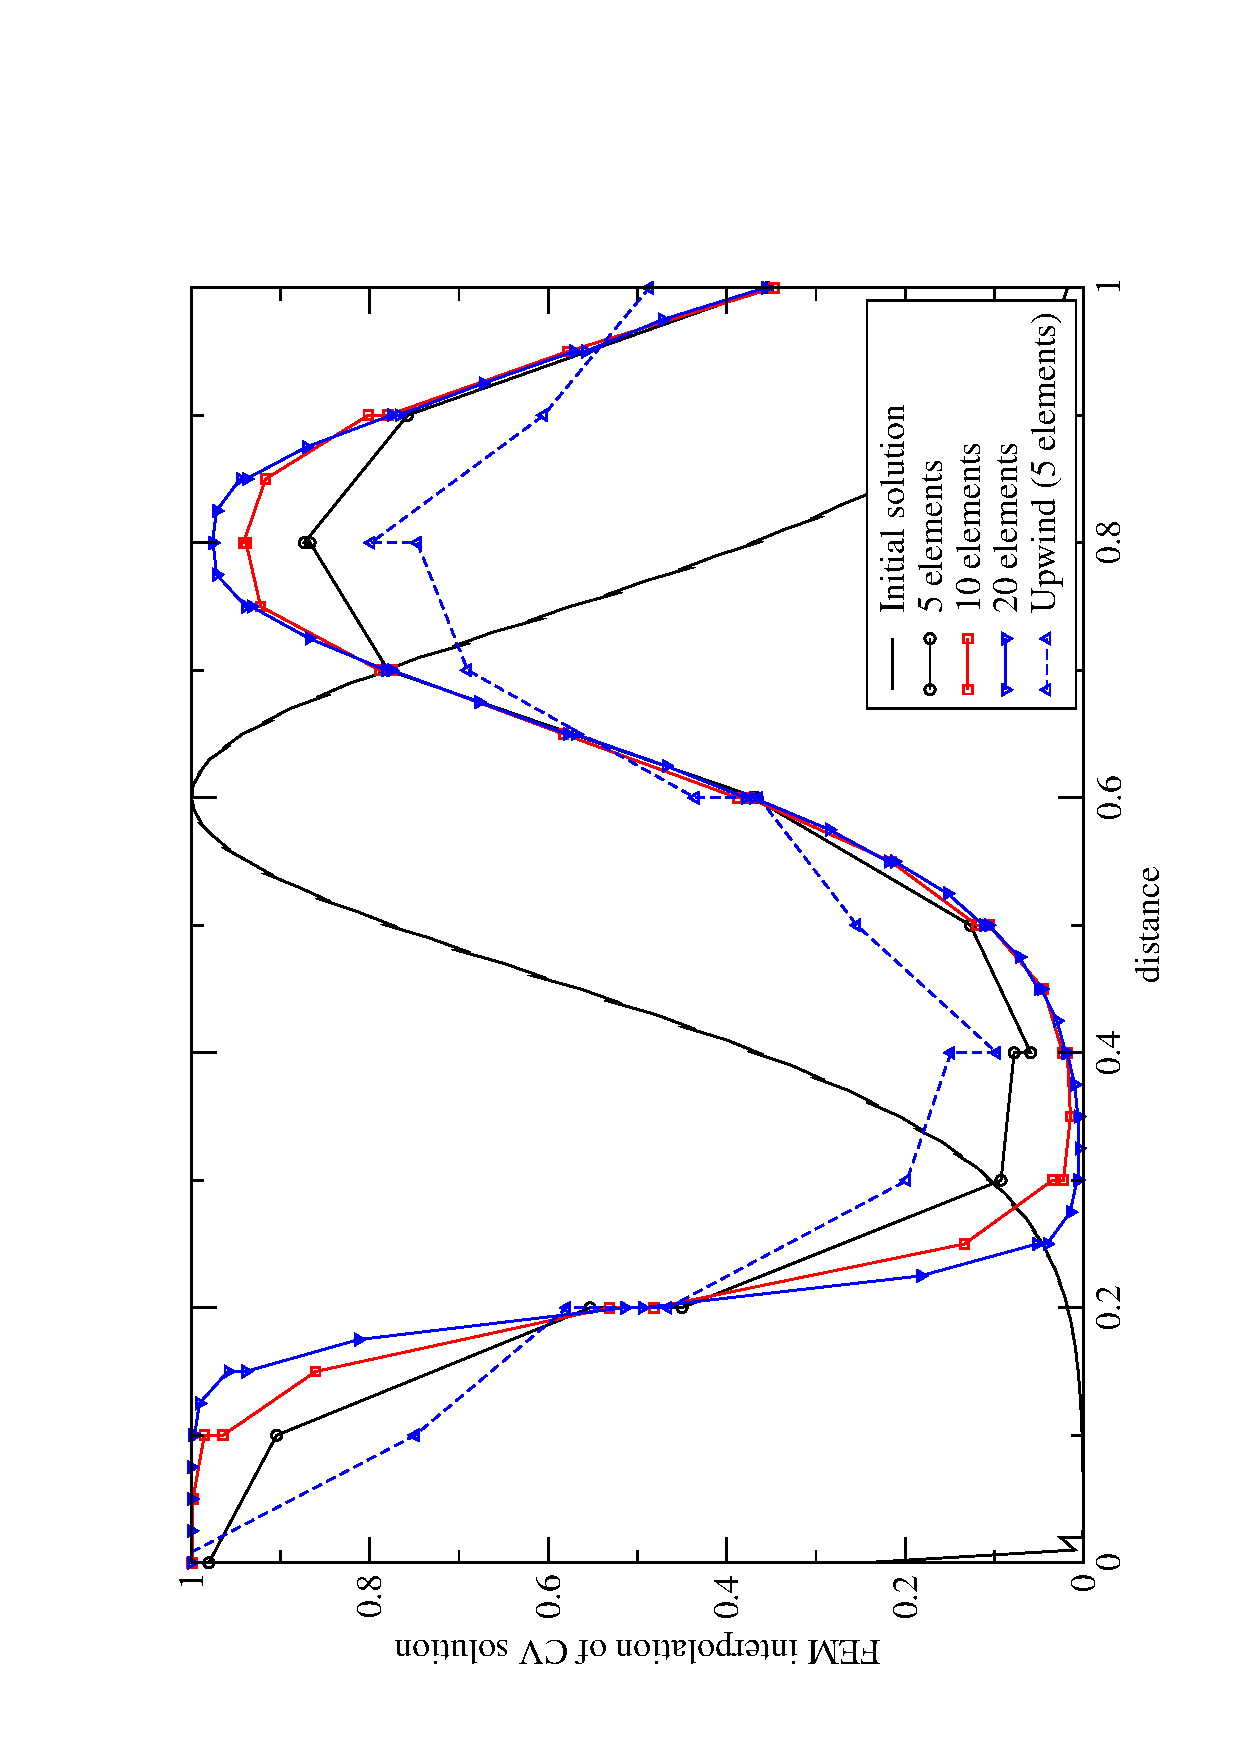
\includegraphics[width=14.0cm,height=10.cm]{converg-fem}}
}\vspace{-.3cm}
\caption{Advection problem test-cases: convergence of the solutions
  with discontinuity between elements and with increased resolution. A
  pure advection problem (from left to right) - the Courant number is
  0.005. The solution has been advected a distance of 0.2. Control
  volume solutions (top) and FEM interpolation (bottom) of the control
  volume solutions are shown. \label{converg}}
\end{figure}


%%%
%%%  FIGURE 
%%%
\begin{figure}[h]
\hbox{\hspace{-1cm}
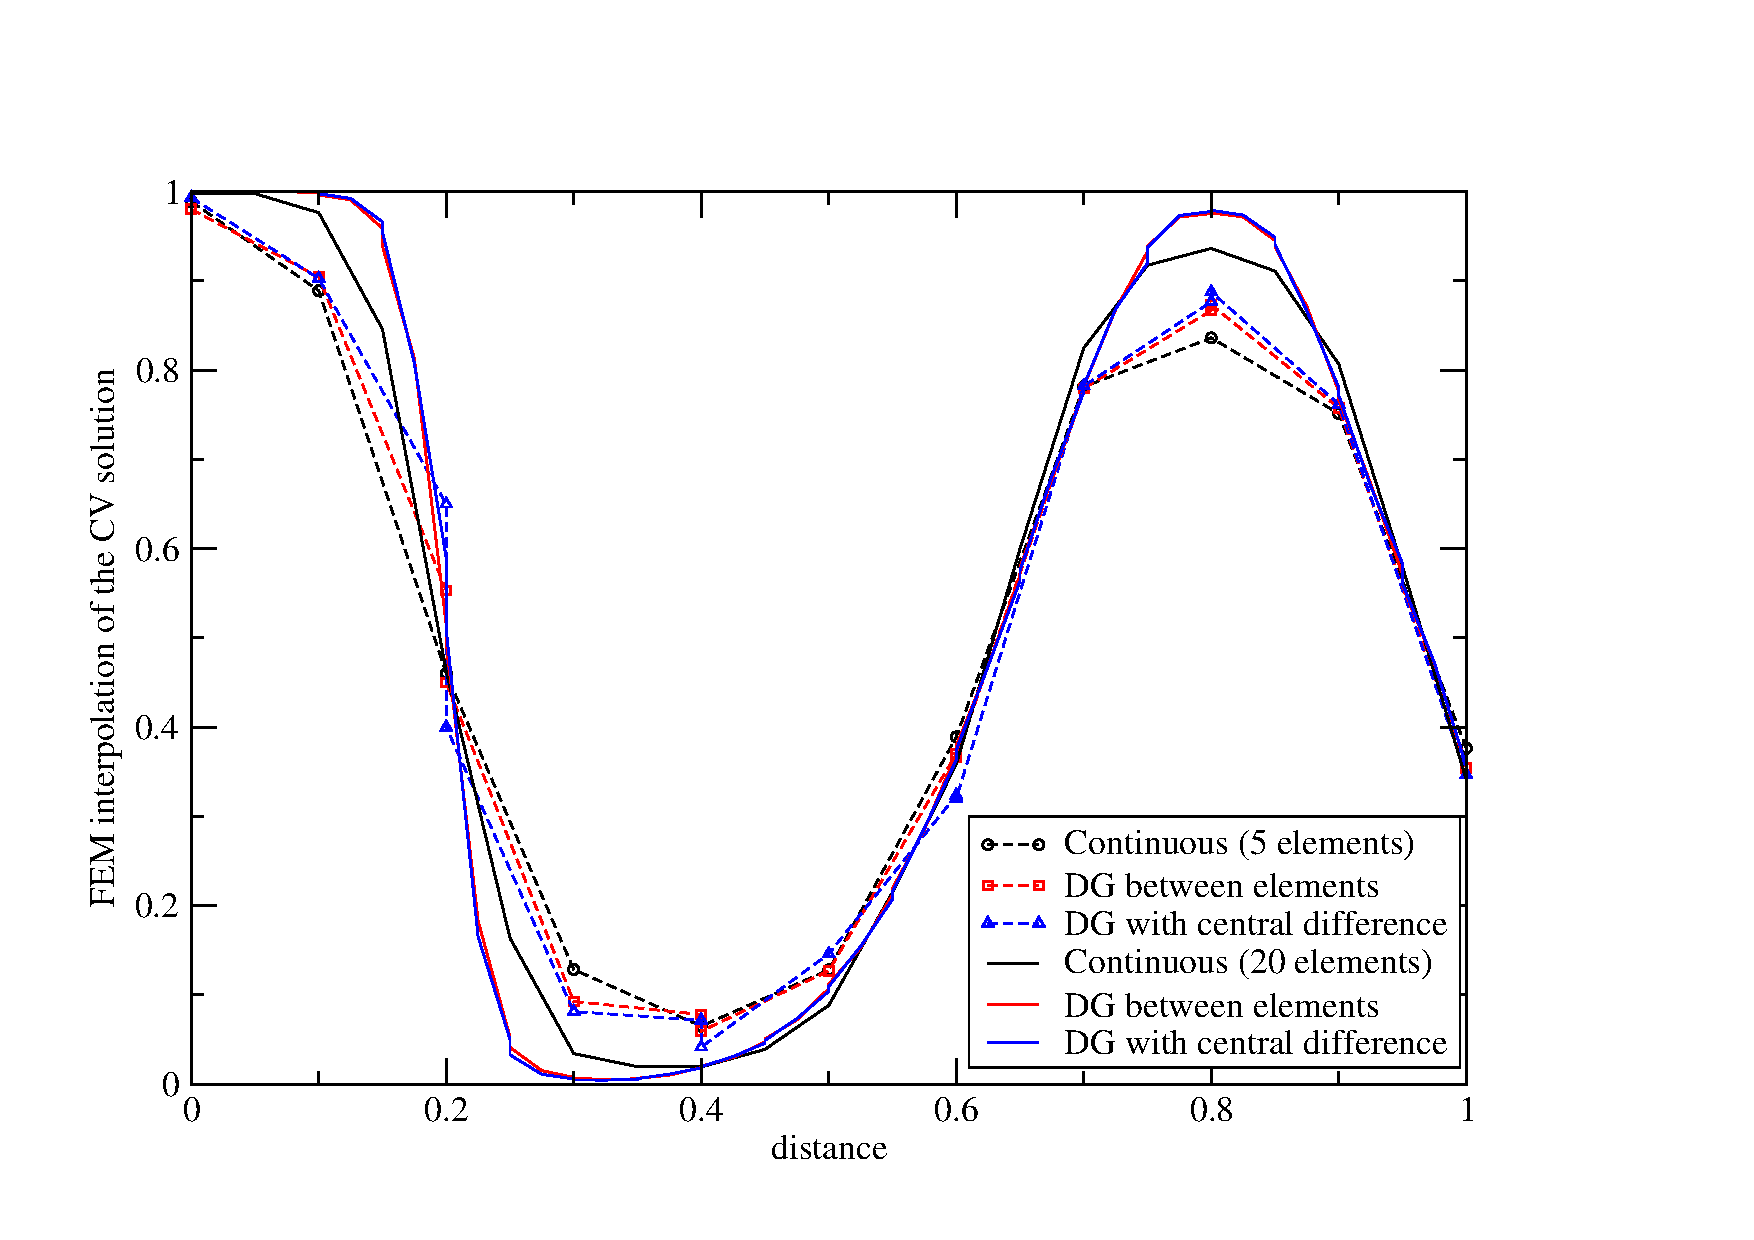
\includegraphics[width=17.5cm,height=12.5cm]{converg-compare-fem}}
\caption{Advection problem test-cases: comparison of convergence of
  the solutions with and without discontinuity between elements and
  with an upwind and central difference flux between the elements and
  with increased resolution (dashed line: 5 elements, full line: 20
  elements). A pure advection problem (from left to right) - the
  Courant number is 0.005. The solution has been advected a distance
  of 0.2. The FEM interpolation of the control volume solutions are
  shown. \label{converg-compare-fem}}
\end{figure}

\begin{comment}
%%%
%%%  FIGURE 
%%%
\begin{figure}[h]
\begin{center}
%\vbox{
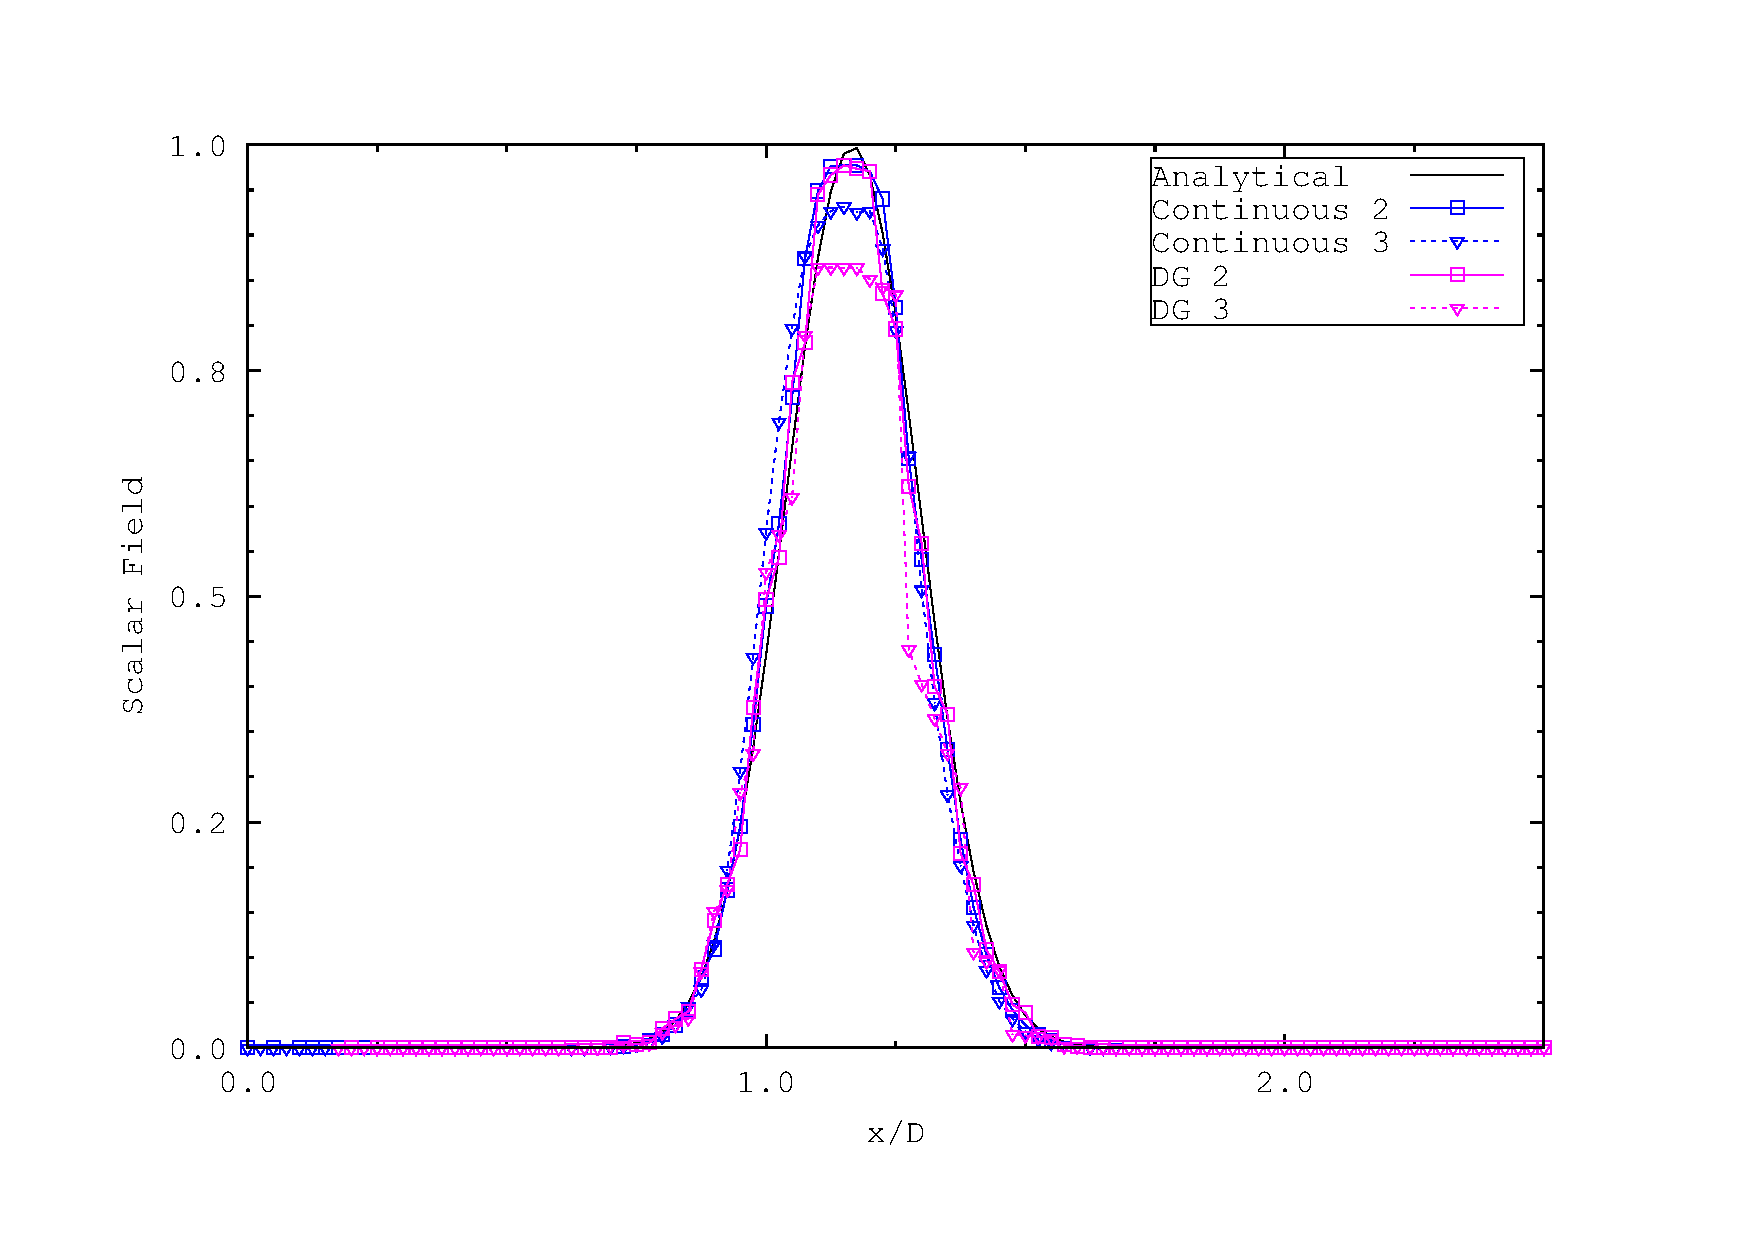
\includegraphics[width=15.5cm,height=12.cm]{./diagrams/Fields_Plume.pdf}
%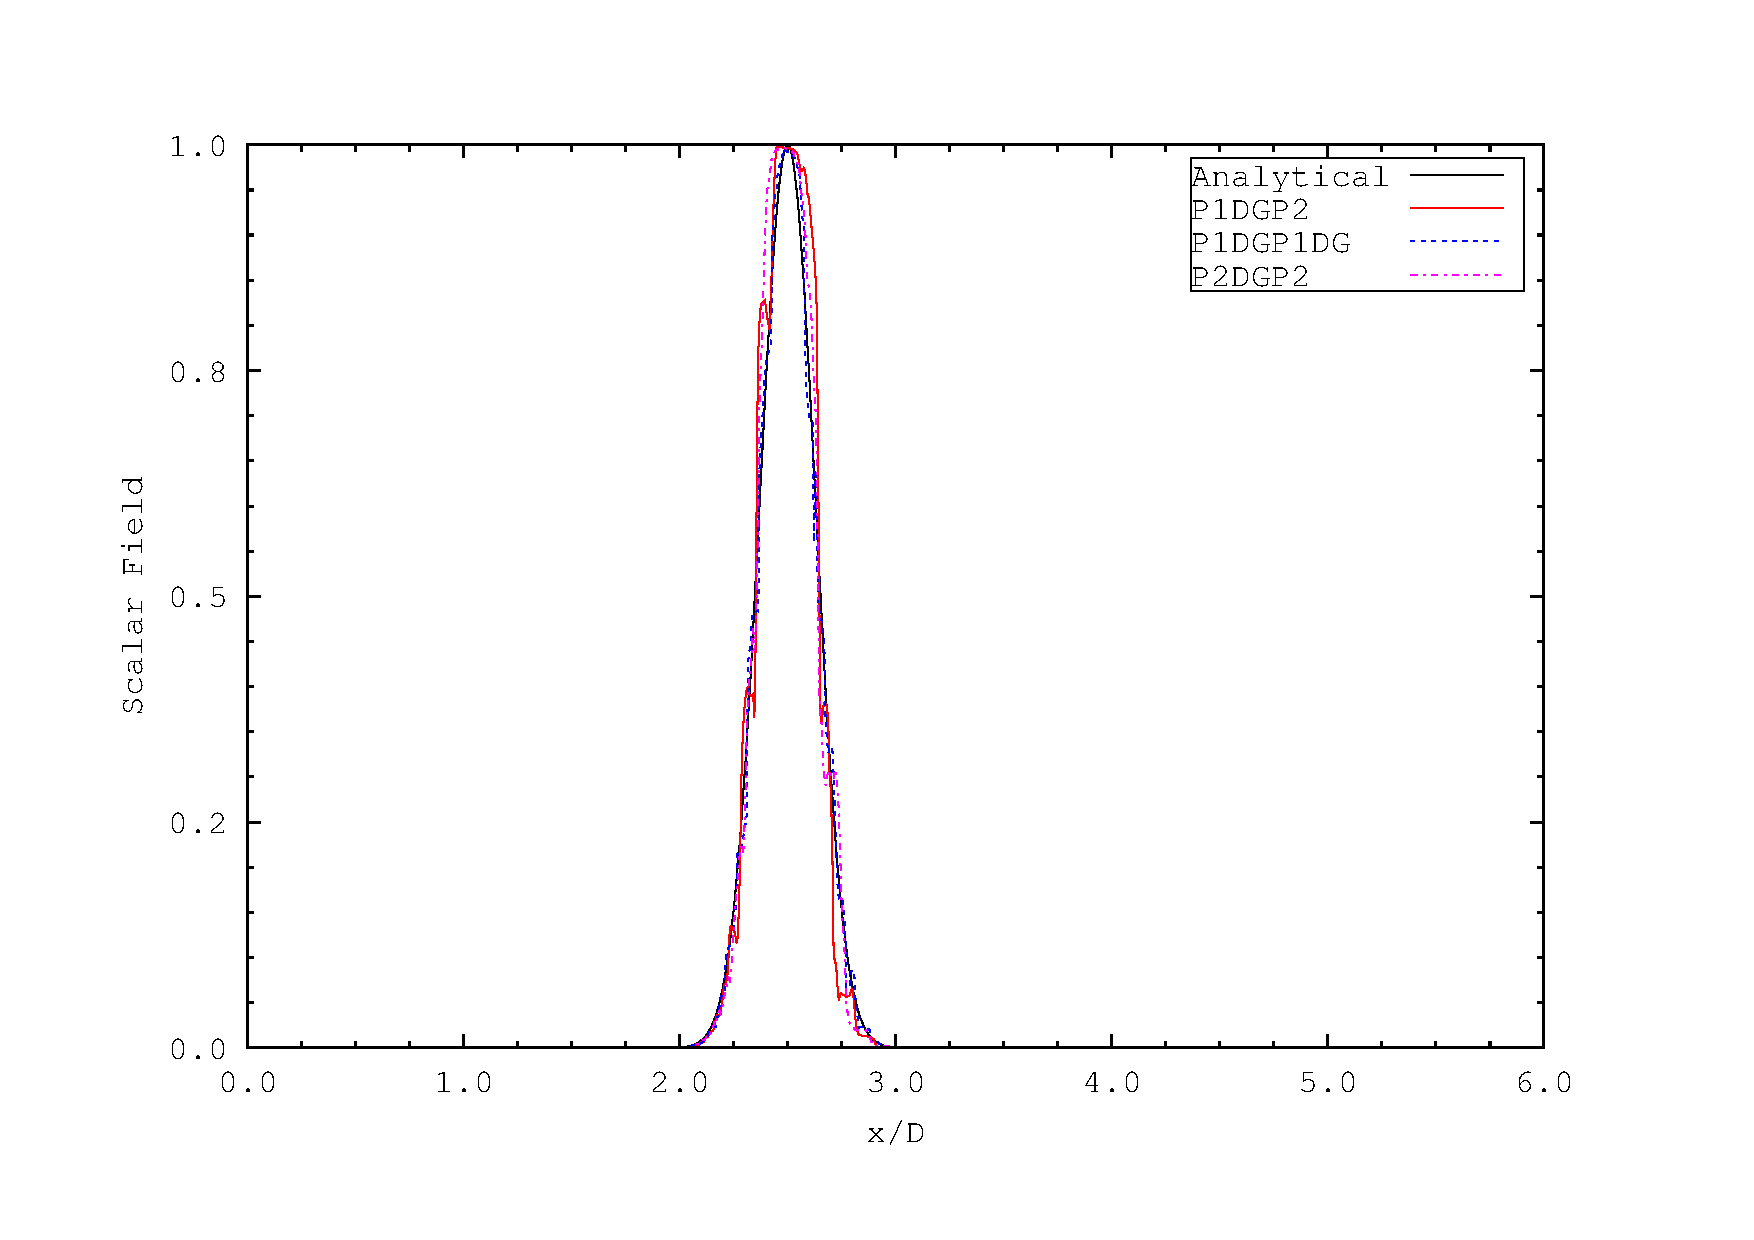
\includegraphics[width=15.5cm,height=12.cm]{./diagrams/AllHighRes.pdf}
%\vspace{-1.5cm}
%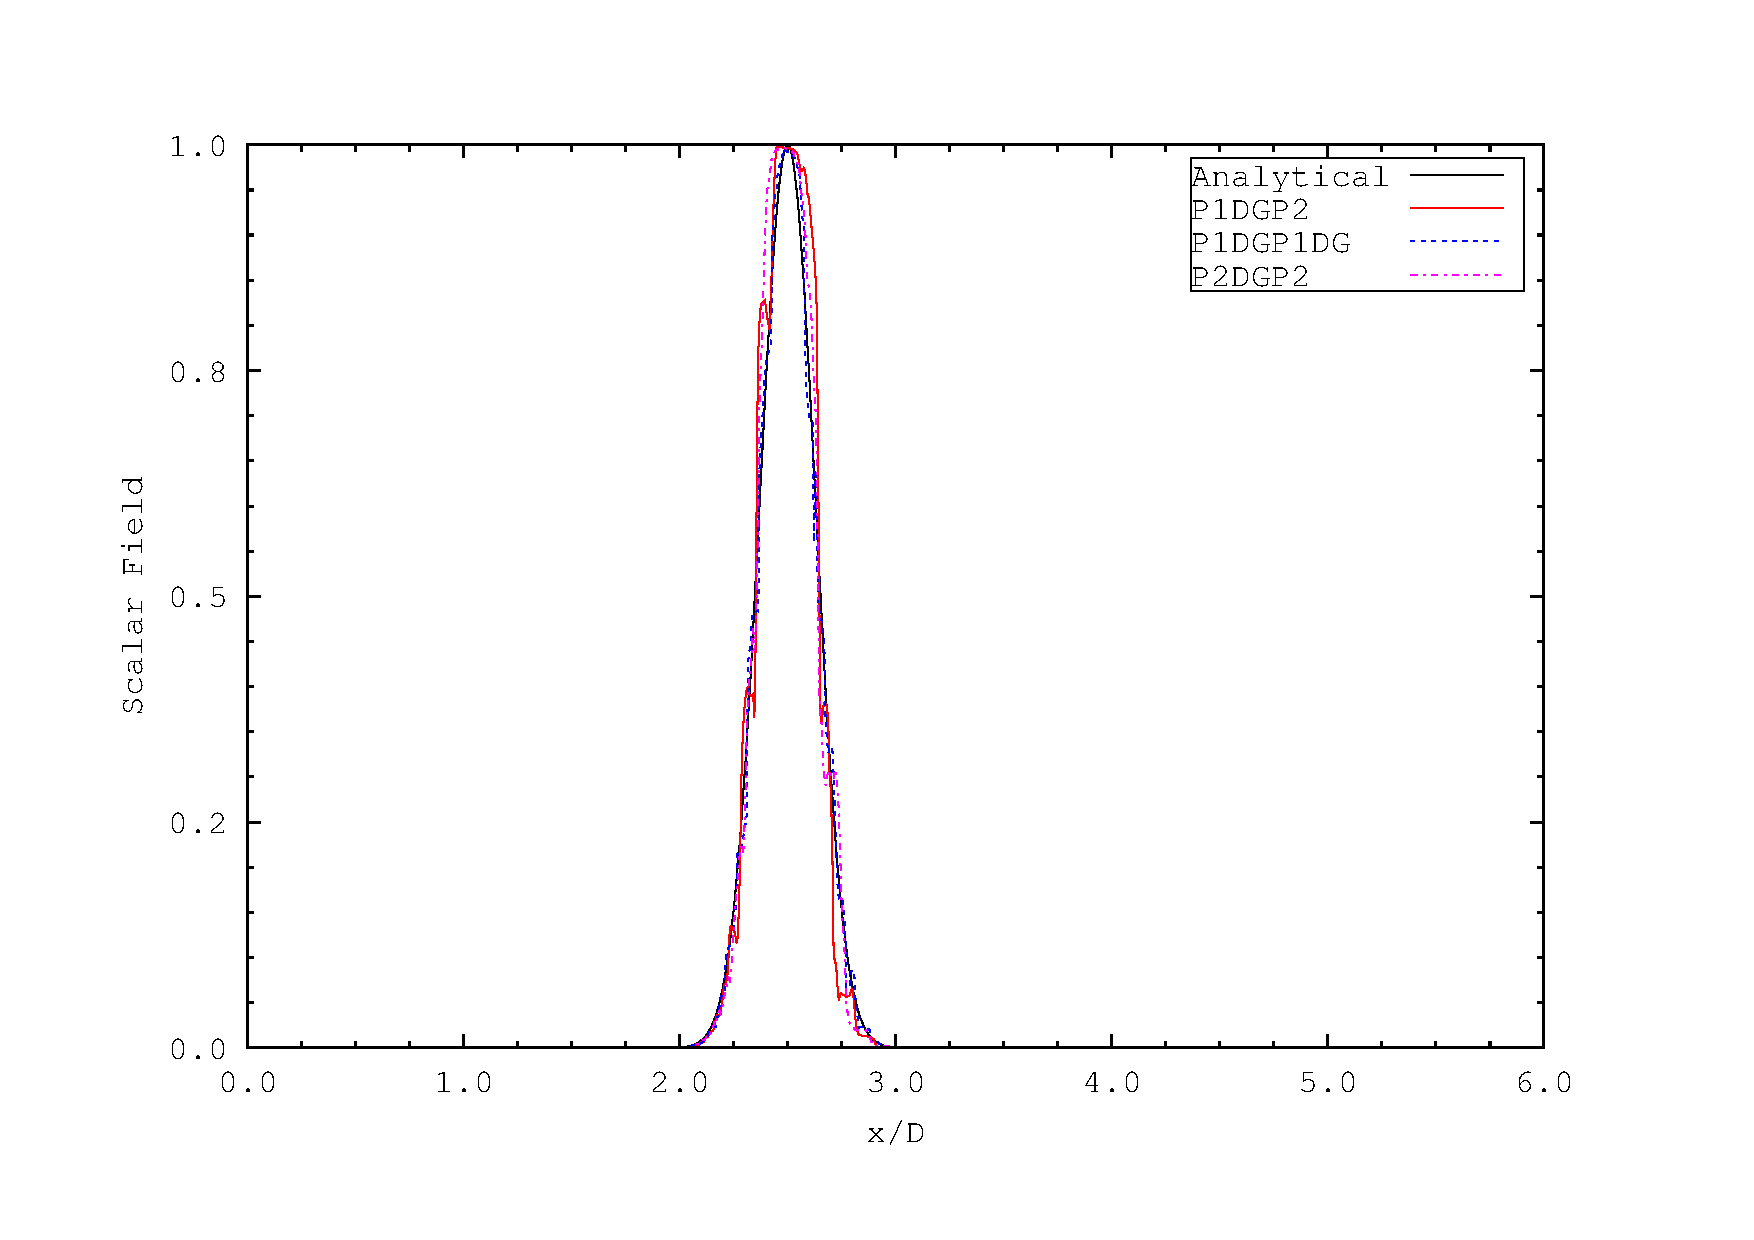
\includegraphics[width=12.5cm,height=9.cm]{./diagrams/AllHighRes.pdf}}
%\vspace{1.cm}
\caption{Advection problem test-cases: Comparison of the resulting 2D advected field after 100 time-steps using continuous and discontinuous (between elements) formulations, in which (2): element size of 0.05 ($\sim$46 elements) and (3): element size: 0.10 ($\sim$ 11 elements).\label{2D_Sanpshot_Adv2D}}
%P$_{1}$DG-P$_{2}$, P$_{2}$DG-P$_{2}$ and P$_{1}$DG-P$_{1}$DG finite elements. There are 11.5k nodes within 22.5k elements. \label{2D_Sanpshot_Adv2D}}
%\caption{Advection problem test-cases: Comparison of the resulting 2D advected field at $t = 0.5$ (500 time-steps) for P$_{1}$DG-P$_{2}$, P$_{2}$DG-P$_{2}$ and P$_{1}$DG-P$_{1}$DG finite elements. There are 11.5k nodes within 22.5k elements. \label{2D_Sanpshot_Adv2D}}
\end{center}
\end{figure}
\end{comment}

%%%
%%%  FIGURE 
%%%
\begin{figure}[h]
\begin{center}
\vbox{\vspace{-1.5cm}\hbox{
\includegraphics[width=15.5cm,height=10.cm]{./diagrams/Step_P1DG-P2Cont}}
\vspace{-.5cm}
\hbox{
\includegraphics[width=15.5cm,height=10.cm]{./diagrams/Plume_P1DG-P2Cont}}}\vspace{-1cm}
\caption{Advection problem test-cases: Comparison of the resulting 2D advected field after 350 (top: step function) and 100 (bottom: Gaussian plume function) time-steps (high-resolution mesh as reference case for time-step size) using continuous and discontinuous (between elements) formulations. Mesh grids used in these simulations are described in Table~\ref{table:meshplume}.\label{2D_Sanpshot_Adv2D}}
%P$_{1}$DG-P$_{2}$, P$_{2}$DG-P$_{2}$ and P$_{1}$DG-P$_{1}$DG finite elements. There are 11.5k nodes within 22.5k elements. \label{2D_Sanpshot_Adv2D}}
%\caption{Advection problem test-cases: Comparison of the resulting 2D advected field at $t = 0.5$ (500 time-steps) for P$_{1}$DG-P$_{2}$, P$_{2}$DG-P$_{2}$ and P$_{1}$DG-P$_{1}$DG finite elements. There are 11.5k nodes within 22.5k elements. \label{2D_Sanpshot_Adv2D}}
\end{center}
\end{figure}



%%%
%%%  FIGURE 
%%%
\begin{figure}[h]
\vbox{\vspace{-2.4cm}
\hbox{
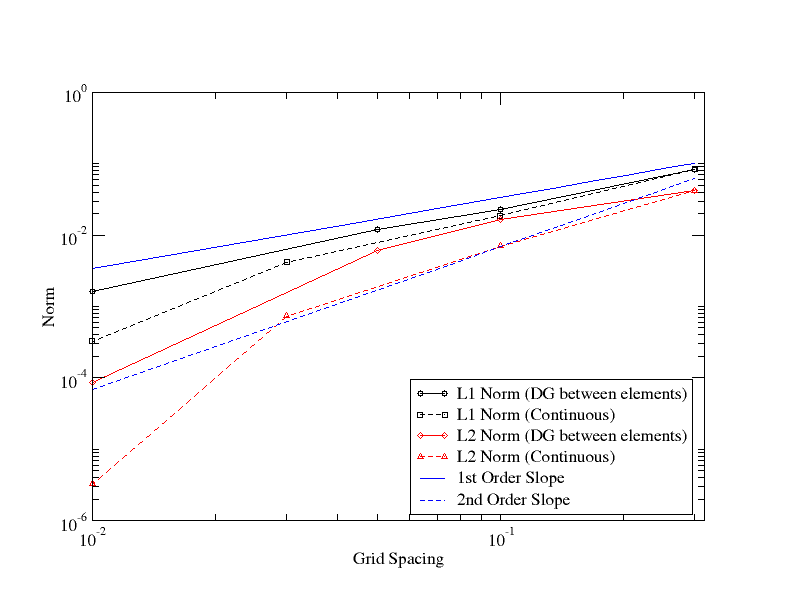
\includegraphics[width=12.5cm,height=10.5cm]{./diagrams/AllNorms_Step.png}}
\vspace{-.4cm}
\hbox{
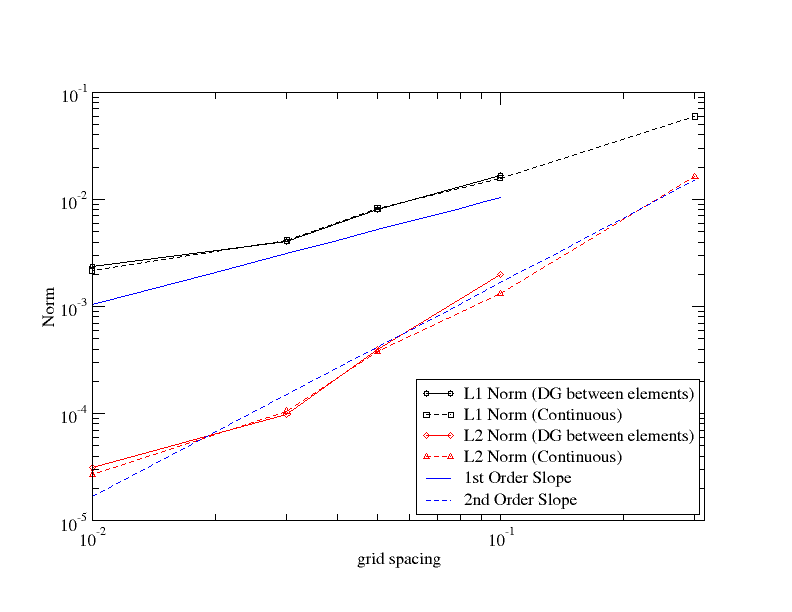
\includegraphics[width=12.5cm,height=10.5cm]{./diagrams/AllNorms2.png}}}
\caption{Advection problem test-cases: comparison of convergence, $L_{1}$ and $L_{2}$ norms for 2D solutions obtained from continuous and discontinuous (between elements) formulations -- top: step funtion; bottom: Gaussian plume function. First- and second-order slopes are also shown in here.\label{L1_L2norm_Adv2D}}
%\caption{Advection problem test-cases: comparison of convergence, $L_{1}$ (top) and $L_{2}$ norms for 2D solutions obtained with $\left(\text{P}_{1}\text{DG-P}_{2}\right.$ and $\left.\text{P}_{2}\text{DG-P}_{2}\right)$ and without $\left(\text{P}_{1}\text{DG-P}_{1}\text{DG}\right)$ discontinuity between elements. \label{L1_L2norm_Adv2D}}
\end{figure}


\begin{comment}


%%%
%%%  FIGURE 
%%%
\begin{figure}[h]
\begin{center}
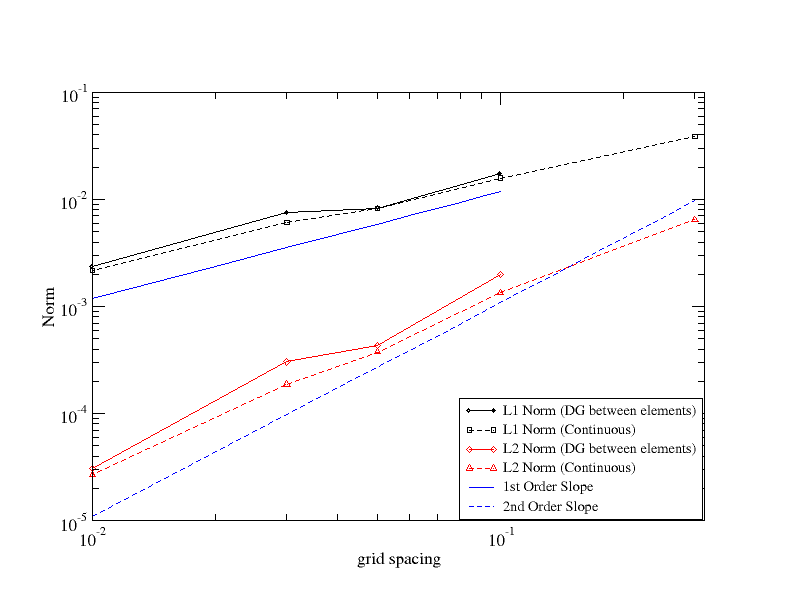
\includegraphics[width=14.5cm,height=13.5cm]{./diagrams/AllNorms.png}
%\begin{center}
%\vbox{
%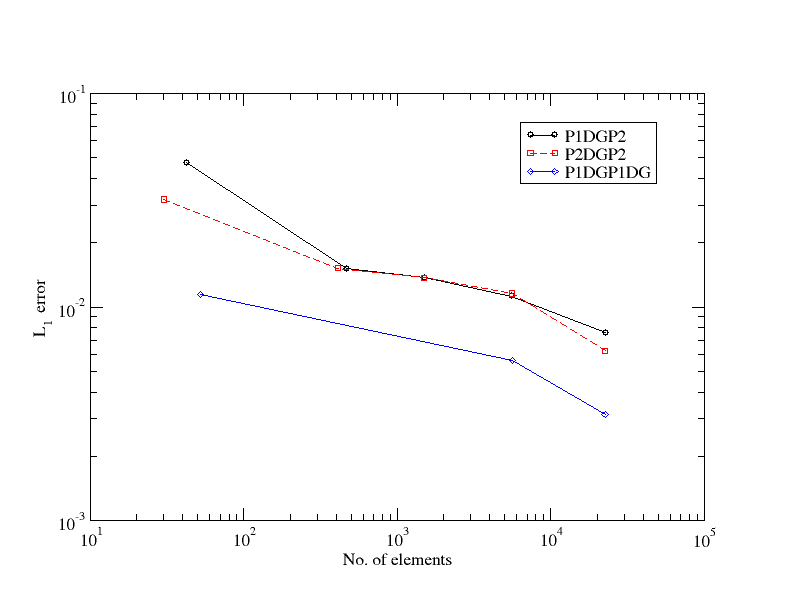
\includegraphics[width=12.5cm,height=9.5cm]{./diagrams/All_L1_PlumeConvergence.png}
%\vspace{-3.cm}
%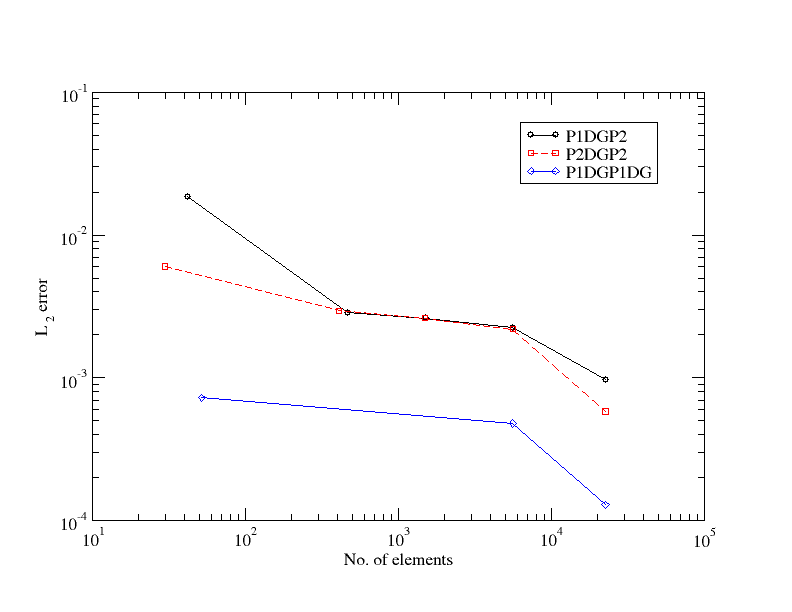
\includegraphics[width=12.5cm,height=9.5cm]{./diagrams/All_L2_PlumeConvergence.png}}
%\vspace{2.cm}
\caption{Advection problem test-cases: comparison of convergence, $L_{1}$ and $L_{2}$ norms for 2D solutions obtained from continuous and discontinuous (between elements) formulations. \label{L1_L2norm_Adv2D}}
%\caption{Advection problem test-cases: comparison of convergence, $L_{1}$ (top) and $L_{2}$ norms for 2D solutions obtained with $\left(\text{P}_{1}\text{DG-P}_{2}\right.$ and $\left.\text{P}_{2}\text{DG-P}_{2}\right)$ and without $\left(\text{P}_{1}\text{DG-P}_{1}\text{DG}\right)$ discontinuity between elements. \label{L1_L2norm_Adv2D}}
\end{center}
\end{figure}


%%%
%%%  FIGURE 
%%%
\begin{figure}[h]
\begin{center}
\includegraphics[width=1.\textwidth]{bl-exact-meth-upwind.eps}
\end{center}
\caption{Buckley--Leverett test-cases: Saturation solutions for the
  continuous upwind method for different 1D P$_{1}$DG-P$_{2}$ mesh
  resolutions and comparison against standard analytical solution.
\label{bl-exact-meth-upwind}}
\end{figure}

%%%
%%%  FIGURE 
%%%
\begin{figure}[h]
  %\begin{center}
\vbox{\hbox{\hspace{2.5cm}
    \includegraphics[width=0.62\textwidth]{BL_1d_P0DGP1_convergence.eps}}
\vspace{-.0cm}\hbox{\hspace{2.5cm}
    \includegraphics[width=0.62\textwidth]{BL_1d_P1DGP2_convergence.eps}}
\vspace{-.0cm}\hbox{\hspace{2.5cm}
    \includegraphics[width=0.62\textwidth]{BL_1d_P2DGP3_convergence.eps}}}
   % 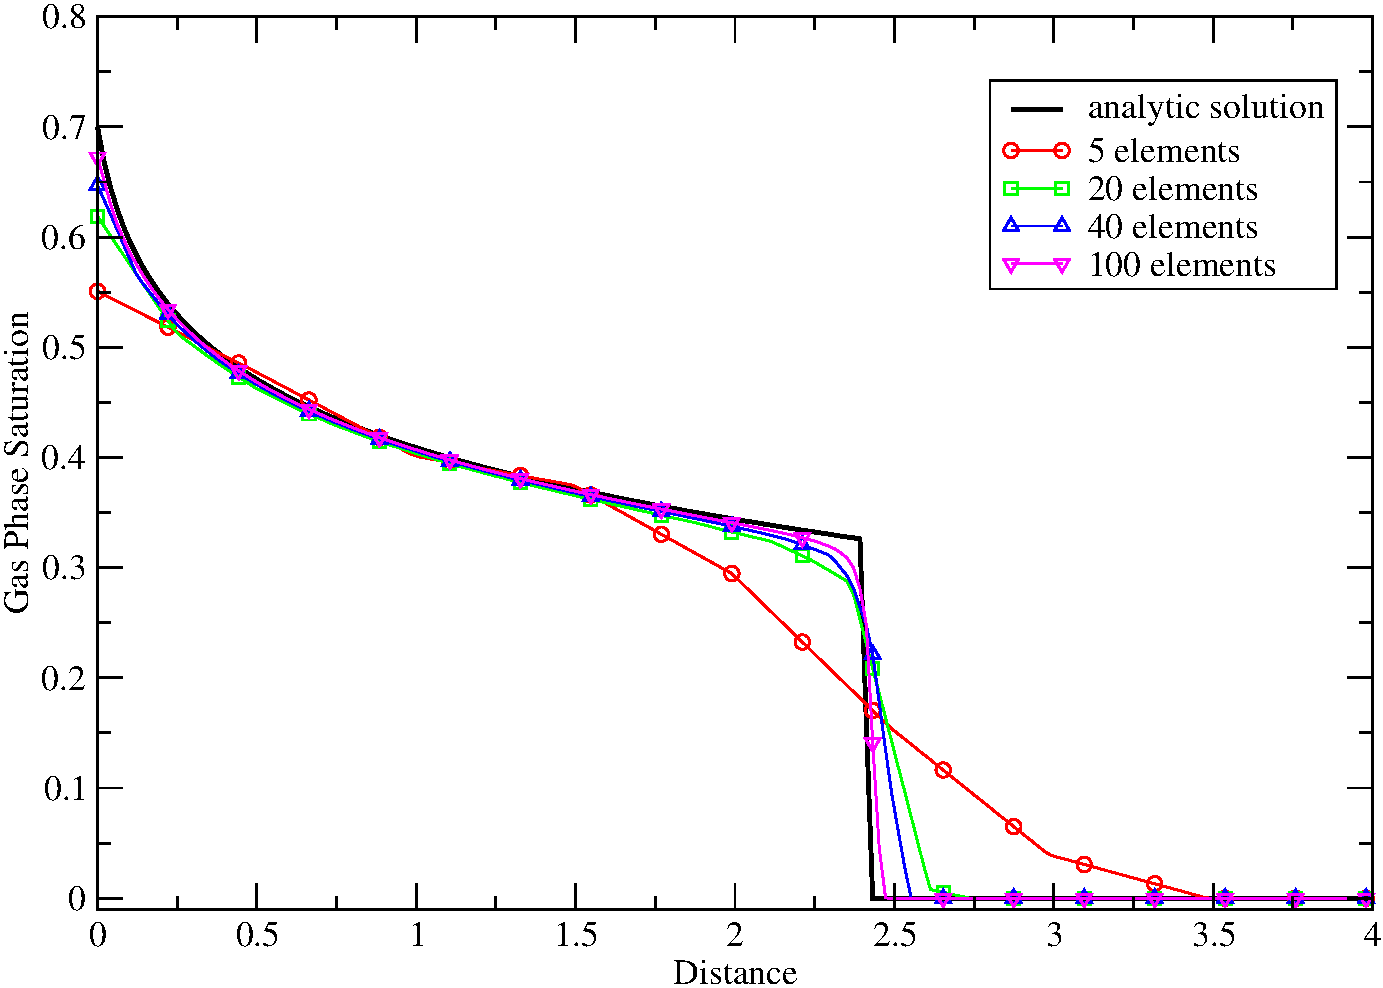
\includegraphics[width=0.45\textwidth]{BL_2d_P1DGP2_convergence}
    \caption{Buckley--Leverett test-cases: Saturation profiles for a
      number of element pairs and numerical resolutions in 1D --
      P$_{0}$DG-P$_{1}$ (top), P$_{1}$DG-P$_{2}$ and P$_{2}$DG-P$_{3}$
      (bottom).\label{fig:BL_profiles}}
  %\end{center}
\end{figure}

%%%
%%%  FIGURE 
%%%
\begin{figure}[h]
\vbox{\hbox{\hspace{1.cm}
    \includegraphics[width=0.8\textwidth]{L1_convergence_rate.eps}}
\vspace{.0cm}\hbox{\hspace{1.cm}
    \includegraphics[width=0.8\textwidth]{L2_convergence_rate.eps}}}
    \caption{Buckley--Leverett test-cases: L1 (top) and L2 (bottom)
      error convergence rates for a number of element
      pairs. \label{fig:BL_converg-rates}}
\end{figure}

%%%
%%%  FIGURE 
%%%
\begin{figure}[h]
\begin{center}
\includegraphics[width=1.\textwidth]{bl-upwind-v-up-and-down.eps}
\end{center}
\caption{Buckley--Leverett test-cases: Comparison of the optimal
  upwind formulation when using upwinding (OU) and coupled
  upwind/downwind (OU-D). The finite element interpolation of the
  saturation field $\left(S_{1}\right)$ is shown at different mesh
  resolutions. Downwind seems to detract from the accuracy of the
  solution. \label{bl-upwind-v-up-and-down}}
\end{figure}

%%%
%%%  FIGURE 
%%%
\begin{figure}[h]
\vbox{
\begin{center}
\includegraphics[width=1.\textwidth]{bl-exact-meth-cv-0-8-ele50.eps}
\end{center}
\vspace{0.cm}}
\caption{Buckley--Leverett test-cases: Comparison of control volume
  solutions using 80$\%$ upwinding and with optimal upwinding and
  using 50 continuous P$_{1}$DG-P$_{2}$
  elements. \label{bl-exact-meth-cv-0-8-ele50}}
\end{figure}

%%%
%%%  FIGURE 
%%%
\begin{figure}[h]
\begin{center}
\includegraphics[width=1.\textwidth]{bl-dg-2eles.eps}
\end{center}
\caption{Buckley--Leverett test-cases: Two element solution using the
  discontinuous formulation. Saturation field from both CV solution
  and FEM interpolation are shown.  \label{bl-dg-2eles}}
\end{figure}

%%%
%%%  FIGURE 
%%%
\begin{figure}[h]
\vbox{
\hbox{\hspace{.3cm}\includegraphics[width=.9\textwidth]{bl-dg-4-10-20.eps}}
\vspace{-0.cm}
\hbox{\hspace{.3cm}\includegraphics[width=.9\textwidth]{bl-dg-cent-4-10-20.eps}}}
\caption{Buckley--Leverett test-cases: Saturation field obtained from
  the discontinuous and continuous formulation with different mesh
  resolutions. Solutions with (top) and without (bottom) upwinding
  scheme. Notice that oscillations are suppressed with the upwinding
  scheme.\label{bl-dg-cent-4-10-20}}
\end{figure}


%%%
%%%  FIGURE 
%%%
\begin{figure}[h]
\vbox{
\hbox{\hspace{.3cm}\includegraphics[width=.9\textwidth]{bl-dg-4-10-vers-cty.eps}}
\vspace{-0.cm}
\hbox{\hspace{.3cm}\includegraphics[width=.9\textwidth]{bl-dg-p1-2-4-5-10-20-40.eps}}}
\caption{Buckley--Leverett test-cases: Saturation field obtained from
  (top) continuous and discontinuous (between elements) formulations
  (solution with 50 elements may be considered as a converged
  result). Solution obtained (bottom) from linear pressure (P1)
  formulation with different mesh resolution with comparison against
  P2-pressure formulation (continuous). \label{bl-dg-4-10-vers-cty}}
\end{figure}


\begin{figure}[H]
\vbox{
\begin{center}
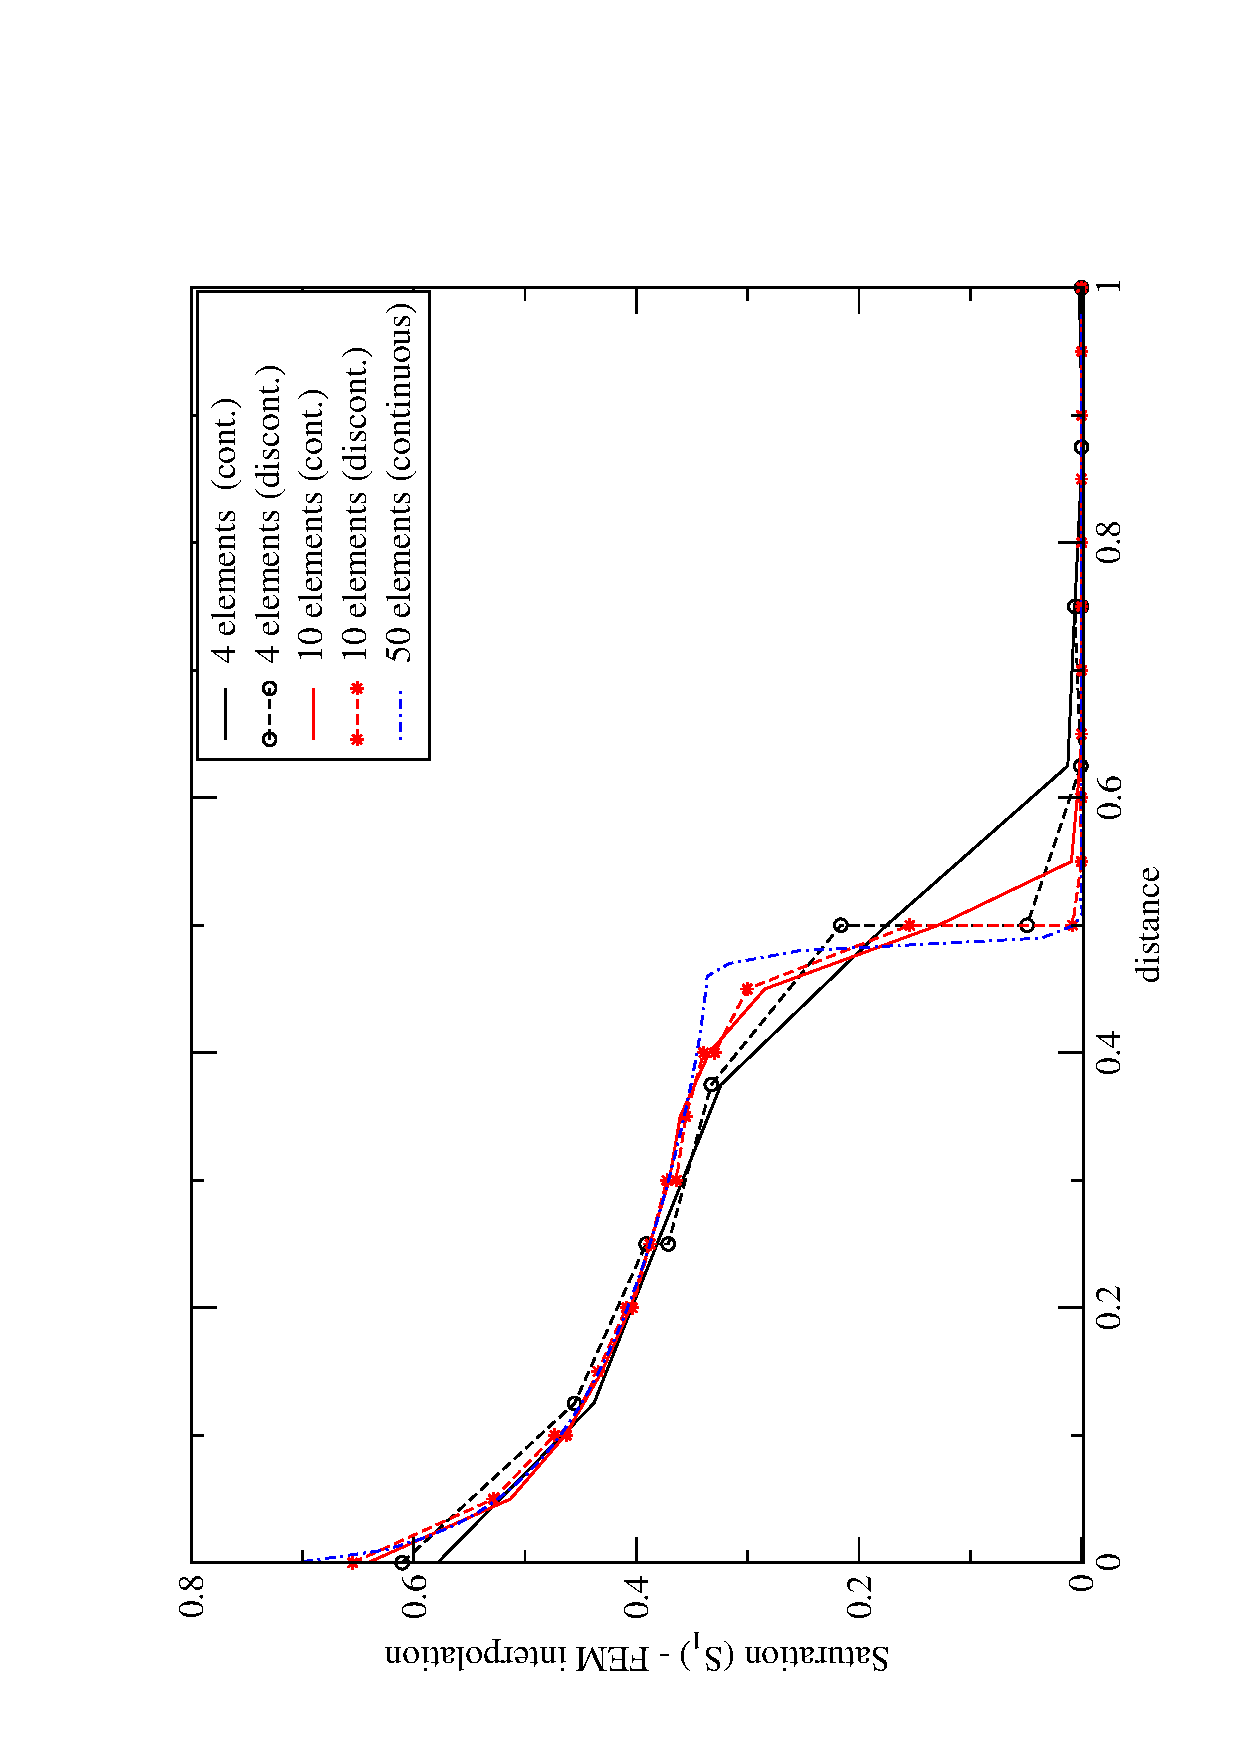
\includegraphics[width=17.5cm,height=12.5cm]{./doc_figures/bl-dg-4-10-vers-cty}
\end{center}
\vspace{0.cm}}
\caption{Gas saturations shown comparing the accuracy of the
  discontinuous between elements and continuous formulation. The 50
  element continuous solution may be viewed as a converged result.  }
\label{bl-dg-4-10-vers-cty}
\end{figure}

\end{comment}

%%%
%%%  FIGURE 
%%%

%%%
%%%  FIGURE 
%%%
